% SPDX-License-Identifier: CC-BY-SA-4.0
% Author: Matthieu Perrin
% Part: <Nom de la partie>
% Section: <Nom de la section>
% Sub-section: <Nom de la sous-section>  % (facultatif, laisser vide si non utilisé)
% Frame: <Titre de la slide>

\begingroup

\begin{frame}{Ambiguïté des grammaires algébriques}
  \begin{block}{Définitions -- Grammaire algébrique ambiguë}
    Soit $G = \langle \Sigma, \Gamma, S, R \rangle$ une grammaire. 
    \begin{itemize}
    \item $G$ est \structure{algébrique} si $R \subseteq \Gamma \times (\Sigma\cup \Gamma)^\star$
      \begin{itemize}
      \item Le membre gauche de toutes ses règles est réduit à un non-terminal
      \end{itemize}
    \item $G$ est \structure{ambiguë} si deux arbres de dérivation génèrent le même mot.
    \end{itemize}
  \end{block}

    \vspace{-2mm}
  \begin{exampleblock}{Exemple : $\left\{A \rightarrow A + A \mid a\right.$}
    Le mot $\example{a+a+a}$ a deux dérivations :

    \hspace\fill
    \scalebox{.8}{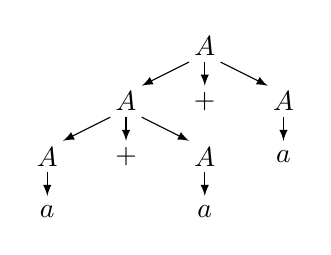
\begin{tikzpicture}
      \draw (5,7.1) node{$A$};
      \draw (4,6.4) node{$A$};
      \draw (5,6.4) node{$+$};
      \draw (6,6.4) node{$A$};
      \draw (3,5.7) node{$A$};
      \draw (4,5.7) node{$+$};
      \draw (5,5.7) node{$A$};
      \draw (3,5.0) node{$a$};
      \draw (6,5.7) node{$a$};
      \draw (5,5.0) node{$a$};

      \draw[-latex] (4.8,6.9) -- (4.2,6.6); 
      \draw[-latex] (5.0,6.9) -- (5.0,6.6); 
      \draw[-latex] (5.2,6.9) -- (5.8,6.6);
      
      \draw[-latex] (3.8,6.2) -- (3.2,5.9); 
      \draw[-latex] (4.0,6.2) -- (4.0,5.9); 
      \draw[-latex] (4.2,6.2) -- (4.8,5.9);
      
      \draw[-latex] (3.0,5.5) -- (3.0,5.2); 
      \draw[-latex] (5.0,5.5) -- (5.0,5.2); 
      \draw[-latex] (6.0,6.2) -- (6.0,5.9);
    \end{tikzpicture}}
    \hspace\fill
    \scalebox{.8}{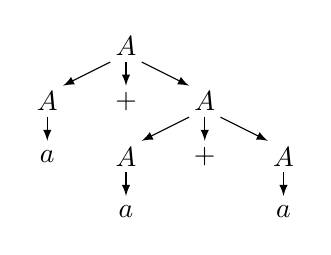
\begin{tikzpicture}
      \draw (5,7.1) node{$A$};
      \draw (4,6.4) node{$A$};
      \draw (5,6.4) node{$+$};
      \draw (6,6.4) node{$A$};
      \draw (5,5.7) node{$A$};
      \draw (6,5.7) node{$+$};
      \draw (7,5.7) node{$A$};

      \draw (4,5.7) node{$a$};
      \draw (5,5.0) node{$a$};
      \draw (7,5.0) node{$a$};

      \draw[-latex] (4.8,6.9) -- (4.2,6.6); 
      \draw[-latex] (5.0,6.9) -- (5.0,6.6); 
      \draw[-latex] (5.2,6.9) -- (5.8,6.6); 
      \draw[-latex] (5.8,6.2) -- (5.2,5.9); 
      \draw[-latex] (6.0,6.2) -- (6.0,5.9); 
      \draw[-latex] (6.2,6.2) -- (6.8,5.9); 
      \draw[-latex] (4.0,6.2) -- (4.0,5.9);
      \draw[-latex] (5.0,5.5) -- (5.0,5.2);
      \draw[-latex] (7.0,5.5) -- (7.0,5.2);
    \end{tikzpicture}}
    \hspace\fill
    \hspace\fill
  \end{exampleblock}

  \vspace{-2mm}
  \begin{block}{Théorème -- Indécidabilité de l'ambiguïté}
    Savoir si une grammaire $G$ est ambiguë est un problème indécidable.
  \end{block}
\end{frame}
\endgroup
